\section{Introduction  }\label{sec:intro}
{\color{blue}[[EDITABLE]]}
%****NOTES START HERE****


%BRAINSTORMING
%\begin{itemize}
%\item Complexity need not be hard to predict (can %point at the simple predictions paper) [[move to %introduction]]
%\item random walk for example is best predicted by %guess what just happend[[move to introduction]]
%\item The kind of complexity present matters, i.e., %that is whether the complexity is structured or not.%[[use here and mention in intro]]






%\item \col brings about the point nicely that some %prediction strategies cannot utilize the processes internal information transfer method. That is a nonlinear internal information transfer system cannot be predicted effectively with a linear strategy. This gives a practitioner leverage on when to give up and when to keep working. [[use in this section as bridge to next section]]

%\end{itemize}



%\begin{it}
%Paragraph on computer performance, including citations to Todd paper
%and summary of the results that indicate that they're deterministic
%nonlinear dynamical systems.  Given that, we should be able to
%predict.  What benefits would accrue if we could do so: power mgmt,
%end world hunger [[this is my primary goal everyday :)]], etc.
%\end{it}
%Things to add to introduction
%\begin{enumerate}

%\item \cmark Make an argument that Computer Performance %is a great testing ground as it gives signals that completely cover the spectrum of complexity \col \dots \gcc

%\item When deterministic structure even complex structure exists that structure can be utilized for prediction.
%\item For noisy real-valued time series distinguishing randomness (WN,RW) complexity from structured nonlinear / chaotic /high period / high dimensional etc complexity is (until now) very hard.
%\subitem for this provide predictions of \gcc and \col side by side and discuss "How can we tell if we did a bad job because the method is inadequate vs the signal being too complex. Lead this into is it possible to tell if there exists structure in a time series to know if we should find a better model or not. Maybe even having 4 predictions. top being ARIMA of the above signals and bottom being LMA of the above signals. Show that one improved and one did not. Is it that we used the wrong method to predict or is it that we simply can't predict the signal better than a random walk due to high levels of internal signal complexity.



%\item\cmark Introduce the two main contributions of the paper which are outlined at the begining of the results section

%\end{enumerate}
%\noindent ***NOTES END HERE****
%
%\noindent ****SECTION START****

Complicated time-series data are ubiquitous in modern scientific
research.  The complexity of these data spans a wide range.  On the
low end of this spectrum are time series that exhibit perfect
predictive structure, i.e, signals whose future values can be
successfully predicted from past values.  In situations like this,
there is an underlying process that generates information and/or
transmits it from the past to the future in a perfectly predictable
fashion.  Constant or periodic signals, for example, fall in this
class.  On the opposite end of this spectrum are signals that are what
we call \emph{fully complex}, where the underlying generating process
transmits no information at all from the past to the future.  Some
examples of this are white noise or random-walk processes.  In signals
like this, knowledge of the past gives no insight into the future,
\emph{regardless} of what model one chooses to use.  Signals in the
midrange of this spectrum---e.g., deterministic chaos, high-period
signals [[Liz question: why does the rank of the periodicity force
    them off the low end of the spectrum?  Any periodic signal can be
    decomposed into sine waves, which can be predicted perfectly...]]
with some additive noise---pose interesting challenges from a modeling
perspective.  In these signals, enough information is being
transmitted from the past to the future that an \emph{ideal}
model---one that captures the generating process---can forecast the
future behavior of the observed system with high accuracy.  [[Liz
    question: if there's noise, is that true?]]

Unfortunately, as a corollary of the undecidability of the halting
problem \cite{halting-problem}, there cannot exist \emph{one}
[[universally]] [[across {\sl all} time series?  this seems pretty
    obvious...]] ideal forecasting scheme for even completely
noise-free deterministic time series\cite{weigend-book}---let alone an
arbitrary real-world time series.  This naturally leads to an
important and challenging question: given a complicated real-valued
time series, does there exist a forecast model that can utilize the
information (if any) that is being transmitted from past to future by
the underlying generating process?  A first step in answering this
question is to reliably quantify where on the complexity spectrum a
given time series falls; a second step is to determine how complexity
and predictability are related.  These are the goals of this paper.

In particular, we wish to determine---without knowing anything about
the generating process---whether a time series is too complex to
predict.  An important practical corollary to this is assessment of
forecast methods: if the forecast produced by a particular method is
poor but the time series contains a significant amount of predictive
structure, the method is inadequate and one should seek another
method.  

We focus on real-valued, scalar, time-series data that appear
\emph{complicated}: i.e., not periodic, linear, constant, etc.  We
make no assumptions about the properties of the generating process:
whether it is linear, nonlinear, deterministic, stochastic,
stationary, non-stationary, etc.  The information in an observation
can be partitioned into two pieces: redundancy and entropy
generation\cite{crutchfield2003}.  Our approach exploits this
decomposition in order to assess how much predictive structure is
present in a signal---i.e., where it falls on the complexity spectrum
mentioned above.  We define \emph{complexity} as a particular
approximation of Kolmogorov-Sinai entropy\cite{KS-entropy}.  That is,
we view a random-walk time series (which exhibits high entropy) as
purely complex, whereas a periodic signal, which exhibits low entropy,
is on the low end of the complexity spectrum.  We argue that an
extension of \emph{permutation entropy} \cite{bandt2002per}---a method
for approximating the entropy through ordinal analysis---is an
effective way to assess the complexity of a given time series.
Permutation entropy is ideal for our purposes because it is known to
converge to the true entropy value, unlike other existing techniques,
which either require specific knowledge of the generating process or
produce biased values of the entropy~\cite{bollt2001}.

To explore the relationship between complexity, predictive structure,
and predictability, we generate forecasts of a number of time-series
datasets using four different prediction methods, then compare the
accuracy of those predictions to the permutation entropy of the
associated signals.  This results in two primary findings:
\begin{enumerate}
\item The complexity of a noisy real-valued time series is
  quantifiable by permutation entropy and correlated with prediction
  accuracy of an ideal predictor [[we don't know that.  we only tried
      four methods.]]
\item The way information is generated and processed internally by a
  system plays a crucial role in the success of different forecasting
  schema.
\end{enumerate}
The forecast methods used here were chosen to span the space of
standard prediction strategies, but they do not cover that space
exhaustively.  Our goal here is an empirical assessment of the
relationship between predictability and complexity, not formal results
about a ``best'' predictor for a given time series.  From a
practitioner's standpoint, it would be useful to know {\sl a priori}
if a trace contains enough predictive structure to make it worth
spending the time and effort searching for a good forecast method.  It
would also be useful to know if a given method is inadequate---that
is, if one could do better and should keep searching.

%[[Introduce and make it clear why we choose comp. perf. as test bed.]]

For the purposes of this study, we require a broad array of
time-series datasets that cover the full complexity spectrum.  Rather
than use synthetic data, we study sensor data from computer
performance experiments.  Computers are among the most complex
engineered artifacts in current use.  Modern microprocessor chips
contain multiple processing units and multi-layer memories, for
instance, and they use complicated hardware/software strategies to
move data and threads of computation across those resources.  As a
result, the processor and memory loads during the execution of even a
very simple program can evolve in a very complicated fashion.
Figure~\ref{fig:ipc} shows a performance trace of a three-line loop
that repeatedly initializes the upper triangle of a matrix in
column-major order.
%
 \begin{figure}[htbp]
    \centering
    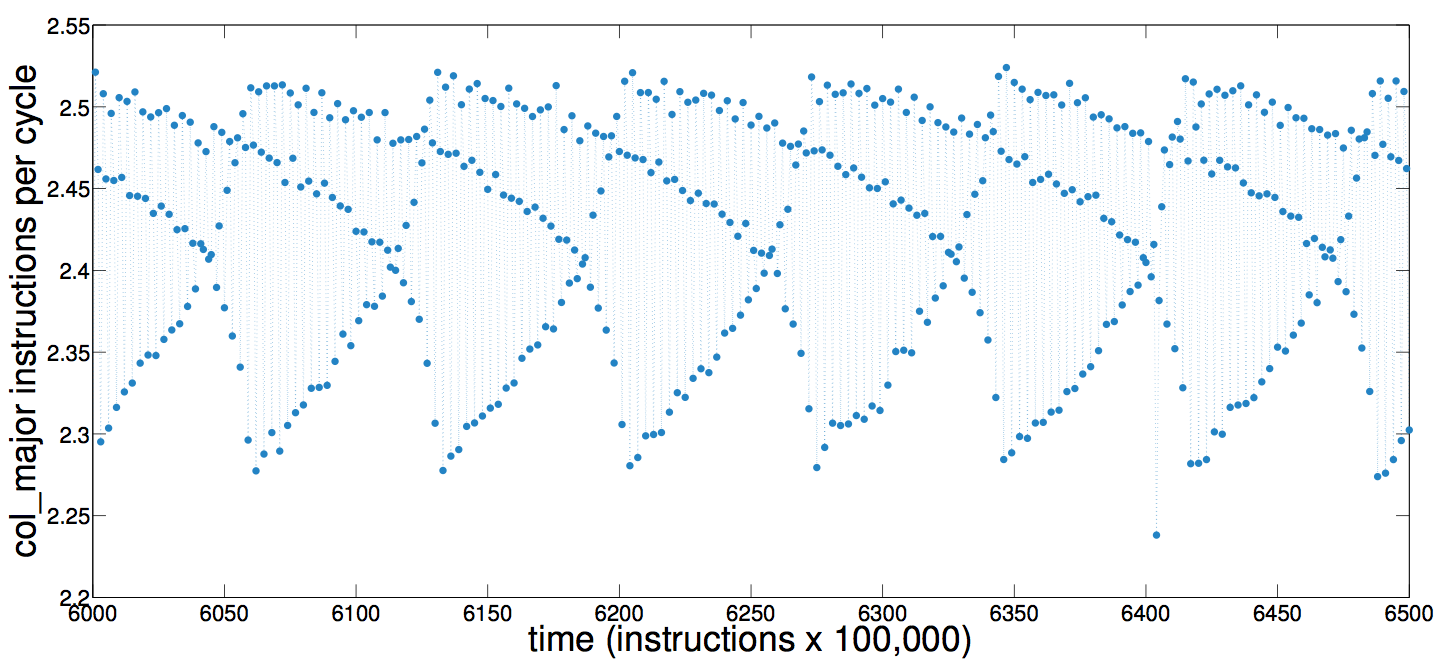
\includegraphics[width=\columnwidth]{figs/colshortts}
    % where an .eps filename suffix will be assumed under latex,
    % and a .pdf suffix will be assumed for pdflatex
    \caption{A computer performance trace: the processor load of \col,
      a three-line C program that repeatedly initializes a matrix in
      column-major order, running on an Intel
      i7\textsuperscript{\textregistered}-based machine.}
   \label{fig:ipc}
  \end{figure}
%
Although this time series appears to be periodic, it is actually
chaotic \cite{mytkowicz09}, which places fundamental limits on
predictability.  Radical changes in this behavior can result if the
program is changed slightly.  The resulting traces span the whole
range of the complexity spectrum, from completely predictable to
completely unstructured, making this an ideal testbed for this study.

%The computer systems community has applied a variety of prediction
%strategies to traces like this, most of which employ regression.  An
%appealing alternative builds on the recently established fact that
%computers can be effectively modeled as deterministic nonlinear
%dynamical systems \cite{mytkowicz09}.  This result %implies the
%existence of a deterministic forecast rule for those %dynamics.  In
%particular, one can use \emph{delay-coordinate %embedding} to
%reconstruct the underlying dynamics of computer %performance, then use
%the resulting model to forecast the future values of computer
%performance metrics such as memory or processor loads
%\cite{josh-ida2011}.  In the case of simple microkernels like the one
%that produced the trace in Figure~\ref{fig:ipc}, this deterministic
%modeling and forecast strategy works very well.  In more-complicated
%programs, however, such as numerical software or compilers,
%this forecast strategy---as well as the traditional methods---break
%down some of the time, but work fine others.

%We argue that \emph{permutation entropy}
%\cite{bandt2002per}, a method for measuring the %entropy of a
%real-valued-finite-length time series through ordinal %analysis, is an
%effective way to explore that conjecture.  %{\color{red} Probably remove this and move a%s it is in the experimental methods or point to that section for more details}We study three
%examples---a simple microkernel and two complex %programs: one from the
%SPEC 2006CPU benchmark suite, and one from LAPACK---%running on an Intel i7-based machine.  For
%each program, we calculate the permutation entropy of %the processor
%load (instructions per cycle), then compare that to %the prediction accuracy attainable for
%that trace using a series of deterministic models.

The rest of the paper is organized as follows:
Section~\ref{sec:related} discusses previous results on [[what]] and
[[what]] and situates this work in that
context. Section~\ref{sec:methods} covers the experimental setup and
methods used to collect each time series. Section~\ref{sec:model}
describes the prediction models we implemented.  In
Section~\ref{sec:meaComplex}, we review weighted permutation entropy.
In Section~\ref{sec:results}, we estimate the complexity of each time
series and compare that complexity to the accuracy of predictions
produced by the methods of Section~\ref{sec:model} on that time
series.  In Section~\ref{sec:conc}, we discuss these results and their
implications and consider future areas of research.

[[Following belongs in the methods section:]] In addition, some
performance traces even exhibit interesting regime changes as a
program switches between varying subroutines. 

[[Following belongs in the conclusion.  Putting it here would be
    appropriate in a CS paper, but not in a physics journal, and not
    when we've just made the point that this is just a testbed.]] 
% paragraph to appease the theoretician in me
It is worth taking a moment to consider the theoretical possibility of
this task. We are not attempting to predict the state of the CPU at an
arbitrary point in the future --- this, at least with perfect
accuracy, would be tantamount to solving the halting problem. What we
are attempting is to predict aspects or functions of the running of
the CPU, e.g., processor efficiency and similar statistics. Prediction
of these quantities at some finite time in the future, even with
perfect accuracy, does not violate the Rice-Shapiro
theorem~\cite{hopcroft} which essentially states that any non-trivial
property of a program is uncomputable.

[[Following is a good start at an abstract. It doesn't need to be
    reiterated in the introduction.]]  This paper provides insight
into when, why, and how forecast strategies fail when they are applied
to complicated time series by empirically estimating their inherent
complexity. [[Liz, do you think here would be better for the sentence
    about we are not the first, or is above where I asked Ryan to
    insert it ok? I worry it would muddy the water of this synopsis
    paragraph.]] We focus here on the specific example of computer
performance but believe the results apply to a much broader class of
time series. We conjecture that the complexity of traces from these
systems---which results from the inherent dimension, non-linearity,
and non-stationarity, as well as from measurement issues like noise,
aggregation, and finite data length---is \emph{empirically
  quantifiable}.  To validate this conjecture we model 120 different
performance traces using a variety of forecasting models.  We then
compare the empirically estimated \emph{complexity} with the accuracy
of each forecast method.
